\documentclass[conference,a4paper]{IEEEtran}
\usepackage{graphicx}
\usepackage{url}
\usepackage{amsmath}
\usepackage[hidelinks]{hyperref}
\renewcommand{\ttdefault}{cmtt}
\graphicspath{{docs/figures/}}
\hypersetup{pdftitle={Instruction and Data Memory Hierarchy},pdfauthor={Team HEXARCH, Section A}}

\title{Instruction and Data Memory Hierarchy:\\A Simple Harvard and von Neumann-Style Comparison}
\author{\IEEEauthorblockN{Akshat Chauhan, Ajeesh Amreet, Vaibhav,\\
Hardik Maheshwari and Mitul Bhatia}
\IEEEauthorblockA{Team HEXARCH, Section A --- MCA Project 9, 2026\\
Newton School of Technology, Rishihood University\\
mitul.bhatia2024@nst.rishihood.edu.in}}

\begin{document}
\maketitle

\begin{abstract}
This paper presents a simplified Harvard memory organization in Verilog and
compares it with a von Neumann-style baseline that uses one shared
single-port memory. Both configurations use the same controller RTL,
program, initial data, 10-ns simulation clock and 32 bytes of storage;
they differ only in one parameter, which selects either separate
instruction and data memories or one shared single-port memory whose
fetch is blocked while it serves a data access. On a three-instruction program
(LOAD, STORE, HALT) the Harvard design completes in four cycles and the
shared design in six, with identical final memory. Across six
self-checking scenarios and 2000 random programs, the measured cycle
counts follow $T_H=N+1$ and $T_S=N+1+M$, where $N$ is the number of
instructions executed and $M$ the number of data accesses. The Harvard
benefit is therefore exactly one cycle per data access, and it vanishes
for programs without data accesses.
\end{abstract}

\begin{IEEEkeywords}
Address decoding, Harvard architecture, instruction fetch, memory
organization, Verilog, von Neumann architecture.
\end{IEEEkeywords}

\section{Introduction}
Instructions tell a controller what operation to perform; data are the
values being used. In a von Neumann (stored-program) machine, both reside
in one memory reached through one path~\cite{vonneumann}, so an
instruction fetch and a data access cannot use that path in the same
cycle~\cite{backus}. A Harvard organization gives instructions and data
separate memories and paths~\cite{aiken}, so the next instruction can be
fetched while the current one reads or writes data.

This project implements both organizations around one small controller
and measures the difference cycle by cycle. It covers instruction/data
separation, address decoding, read/write control, simulation waveforms and
an architecture comparison. The 32-byte shared memory is a comparison
baseline, not a second level of a hierarchy; the brief's optional shared
lower-level memory is not implemented in Phase~I.

\section{Literature Review}
\subsection{Von Neumann and Harvard Organizations}
Von Neumann's 1945 EDVAC report described a stored-program computer whose
instructions and data reside in a single memory~\cite{vonneumann}.
Backus later called the single channel between processor and memory the
``von Neumann bottleneck''~\cite{backus}. The Harvard Mark~I, described
by Aiken and Hopper, instead read its instruction sequence from punched
tape, separate from the registers that held its data~\cite{aiken}.
``Harvard architecture'' now denotes any design with separate instruction
and data storage and paths.

\subsection{Modified Harvard Designs and Split Caches}
Most general-purpose processors keep one unified main memory but split
the first level of the memory hierarchy into instruction and data caches,
so that an instruction fetch and a data access can proceed in the same
cycle~\cite{hp,smith}. When fetch and load/store compete for a single
memory port in a pipeline, the result is a structural hazard that forces
a stall~\cite{hp}. The stall in our shared design is a minimal instance
of this hazard.

\subsection{Microcontroller Practice}
Small embedded processors use Harvard memories directly. Microchip's
enhanced mid-range PIC has independent instruction and data buses and a
two-stage pipeline in which the next instruction is fetched while the
current one executes~\cite{pic}. The AVR core likewise separates program
and data memory and pre-fetches the next instruction during
execution~\cite{avr}. Our single instruction register reproduces this
fetch/execute overlap; the model uses its own four-opcode instruction set
and does not emulate either processor.

\subsection{Design Language and Tools}
The RTL is written in Verilog~\cite{ieee1364}; the self-checking
testbenches use SystemVerilog constructs~\cite{ieee1800}. Both are
compiled and simulated with Icarus Verilog~\cite{icarus}.

\section{Proposed Solution}
\subsection{Memories and Controller}
The Harvard configuration has a $16\times8$-bit instruction memory and a
$16\times8$-bit data memory with independent ports; each decodes its own
four-bit address. The von Neumann-style configuration has one
$32\times8$-bit memory with a single port. Its address decoder maps
instruction offsets to physical addresses 0--15 and data offsets to
16--31. Both hold 32 bytes. Fig.~\ref{fig:architecture} shows the two
organizations; one parameter, \texttt{SHARED\_BUS}, selects between them
in \texttt{memory\_system.v}.

The controller contains a four-bit program counter (PC), an eight-bit
instruction register (IR) with a valid bit, and an eight-bit accumulator
(ACC). The PC advances only when a fetch is accepted, and the IR holds the
current instruction while the PC addresses the next one. The read/write
control module decodes the IR into LOAD, STORE, HALT and illegal; the
controller gates these with the valid bit to drive the data-read and
data-write enables.

\begin{figure}[t]
\centering
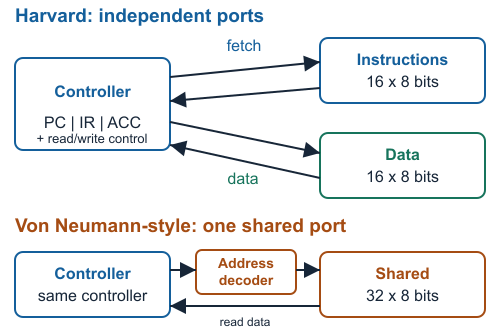
\includegraphics[width=\columnwidth]{architecture_report.png}
\caption{Block diagram. Top: Harvard organization with independent
instruction and data ports; the controller contains the program counter
(PC), instruction register (IR), accumulator (ACC) and read/write
control. Bottom: von Neumann-style baseline, in which the address decoder
forms one 5-bit address for a single-port memory.}
\label{fig:architecture}
\end{figure}

\subsection{Instructions and Timing}
The upper nibble of each instruction selects the operation and the lower
nibble a data address: LOAD (\texttt{1a}) reads data[$a$] into ACC;
STORE (\texttt{2a}) writes ACC to data[$a$]; HALT (\texttt{Fa}) stops;
NOP (\texttt{0a}) performs no data operation. Other opcodes stop with a
fault flag.

Reads are combinational; LOAD captures data and STORE commits its write
at the rising clock edge. A synchronous active-high reset clears the
controller and suppresses memory requests while retaining memory
contents. The 10-ns clock is a simulation setting, not a measured
hardware frequency. Programs must fit in 16 instruction bytes and end in
HALT, because the four-bit PC otherwise wraps.

In Harvard mode, fetching the next instruction overlaps the current LOAD
or STORE. In shared mode, data has priority: fetch is blocked, the PC
holds and the valid bit clears, so the next cycle fetches the delayed
instruction without repeating the previous one. HALT suppresses all
further memory traffic.

\section{Prototype and Verification}
The demonstration program is \texttt{LOAD 0; STORE 1; HALT}, encoded as
\texttt{10 21 F0}. Initially data[0] is 7 and all other data is zero.
Both designs must finish with ACC~$=7$, data[0]~$=7$ and data[1]~$=7$,
with all other data and all instructions unchanged.

\texttt{make demo} prints the cycle-by-cycle table and writes a VCD
waveform. \texttt{make test} runs six scenarios: the demonstration,
boundary addresses (including a STORE immediately followed by a LOAD of
the same address), no data accesses, HALT only, an invalid opcode, and a
reset in the middle of a longer copy sequence. The testbench checks every
final data word, that instructions are unchanged, that each design
performs exactly the expected number of data operations, with the same
read and write counts in both designs, PC advance and hold, exclusive use of the shared port,
and inactivity after HALT. \texttt{make stress} runs 2000 random
straight-line programs on both designs and compares them with a software
model. All checks pass with Icarus Verilog 13.0.

\section{Results and Discussion}
Table~\ref{tab:results} gives the measured cycles, counted from the
first rising edge after reset release up to and including the cycle that
executes HALT (or the invalid opcode).

\begin{table}[t]
\caption{Measured completion cycles. $N$: instructions executed;
$M$: LOAD/STORE count; stalls: blocked shared fetches.}
\label{tab:results}
\centering
\begin{tabular}{lrrrrr}
\hline
Scenario & $N$ & $M$ & Harvard & Shared & Stalls \\ \hline
LOAD 0; STORE 1; HALT & 3 & 2 & 4 & 6 & 2 \\
Address boundaries & 5 & 4 & 6 & 10 & 4 \\
Two NOPs and HALT & 3 & 0 & 4 & 4 & 0 \\
HALT only & 1 & 0 & 2 & 2 & 0 \\
Invalid opcode & 1 & 0 & 2 & 2 & 0 \\
Copy chain after reset & 7 & 6 & 8 & 14 & 6 \\ \hline
\end{tabular}
\end{table}

\begin{figure}[t]
\centering
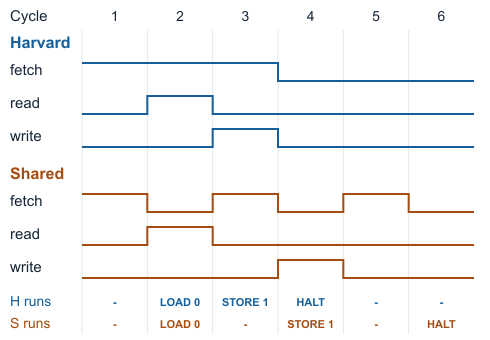
\includegraphics[width=\columnwidth]{waveforms_report.png}
\caption{Demo controls, redrawn from the testbench trace and sampled
before each rising edge, with the instruction each design executes.
Harvard fetch overlaps the data read (cycle 2) and write (cycle 3);
shared fetch is blocked in cycles 2 and 4.}
\label{fig:waveforms}
\end{figure}

In cycle 1 both designs fetch LOAD. In cycle 2 the Harvard design
executes LOAD and fetches STORE; in cycle 3 it executes STORE and fetches
HALT, which executes in cycle 4. The shared design blocks fetch during
LOAD (cycle 2) and STORE (cycle 4) and executes HALT in cycle 6
(Fig.~\ref{fig:waveforms}). Both produce the expected value 7.

\subsection{Cycle Model}
The first cycle after reset only fetches. Every later cycle executes one
instruction, and in the Harvard design it also fetches the next, so
\begin{equation}
T_H = N + 1.
\end{equation}
In the shared design each LOAD or STORE occupies the single port and
moves the following fetch to an extra cycle, so
\begin{equation}
T_S = N + 1 + M, \qquad \frac{T_S}{T_H} = 1 + \frac{M}{N+1}.
\end{equation}
Every row of Table~\ref{tab:results} satisfies both expressions, as did
all 2000 random programs. For the demonstration ($N=3$, $M=2$) the ratio
is 1.5. Because a program that ends in HALT has $M\le N-1$, the ratio
stays below 2, and it equals 1 when $M=0$. The benefit therefore depends
on the workload rather than being a universal speed-up.

\subsection{Limitations}
Memory reads are combinational, which matches asynchronous (distributed)
RAM rather than the synchronous block RAM common on FPGAs; a
synchronous-read memory would add fetch latency that is not modelled.
There are no branches, and synthesis, resource use and maximum clock
frequency have not been measured.

\section{Individual Contributions}
Table~\ref{tab:contrib} lists each member's area of responsibility; each
member presents that part in the prototype video. The initial
implementation was committed by Mitul Bhatia (see the Acknowledgment);
each member's own commits in the project repository record the work they
completed.

\begin{table}[t]
\caption{Responsibilities}
\label{tab:contrib}
\centering
\begin{tabular}{p{0.24\columnwidth}p{0.66\columnwidth}}
\hline
Member & Responsibility \\ \hline
Akshat Chauhan & Instruction path: program counter, instruction memory \\
Ajeesh Amreet & Data path: data memory, read/write control \\
Vaibhav & Shared memory, address decoder, fetch-stall rule \\
Hardik Maheshwari & Simulation: testbenches, results, waveforms \\
Mitul Bhatia & Integration: top level, controller, build, report, repository, video \\ \hline
\end{tabular}
\end{table}

\section{Conclusion}
The prototype separates instruction and data paths in a Harvard
organization and compares it with a single-port von Neumann-style
baseline built from the same controller RTL and storage. Self-checking
simulation shows identical results in both organizations; the Harvard
design saves exactly one cycle per data access ($T_S-T_H=M$), and the
two take the same time for programs without LOAD or STORE. Phase~II can
add the optional shared lower-level memory behind the split memories, a
synchronous-read memory model and synthesis results. Source code,
results and the demonstration video link are in the project repository:
\url{https://github.com/mitul-bhatia/HEXARCH}.

\section*{Acknowledgment}
The Verilog RTL, testbenches, figures and parts of this text were drafted
with the help of an AI assistant and were reviewed, run and checked by
the team. The IEEEtran class by M.~Shell is used under the LaTeX Project
Public License.

\begin{thebibliography}{10}
\bibitem{vonneumann} J. von Neumann, ``First draft of a report on the
EDVAC,'' \textit{IEEE Ann. Hist. Comput.}, vol. 15, no. 4, pp. 27--75,
1993, doi: 10.1109/85.238389.
\bibitem{backus} J. Backus, ``Can programming be liberated from the von
Neumann style? A functional style and its algebra of programs,''
\textit{Commun. ACM}, vol. 21, no. 8, pp. 613--641, Aug. 1978,
doi: 10.1145/359576.359579.
\bibitem{aiken} H. H. Aiken and G. M. Hopper, ``The automatic sequence
controlled calculator---I,'' \textit{Elect. Eng.}, vol. 65, no. 8--9,
pp. 384--391, Aug.--Sep. 1946, doi: 10.1109/EE.1946.6434251.
\bibitem{hp} J. L. Hennessy, D. A. Patterson, and C. Kozyrakis,
\textit{Computer Architecture: A Quantitative Approach}, 7th ed.
Cambridge, MA, USA: Morgan Kaufmann, 2025.
\bibitem{smith} A. J. Smith, ``Cache memories,'' \textit{ACM Comput.
Surv.}, vol. 14, no. 3, pp. 473--530, Sep. 1982,
doi: 10.1145/356887.356892.
\bibitem{pic} Microchip Technology, ``8-bit PIC MCU enhanced mid-range
architectural overview,'' \textit{Developer Help}, Jan. 23, 2024.
[Online]. Available:
\url{https://developerhelp.microchip.com/xwiki/bin/view/products/mcu-mpu/8bit-pic/enhanced-family/mrarch/}.
Accessed: Nov. 8, 2026.
\bibitem{avr} Microchip Technology, ``AVR CPU core,'' \textit{Developer
Help}, Nov. 10, 2023. [Online]. Available:
\url{https://developerhelp.microchip.com/xwiki/bin/view/products/mcu-mpu/8-bit-avr/structure/core/}.
Accessed: Nov. 8, 2026.
\bibitem{ieee1364} \textit{IEEE Standard for Verilog Hardware Description
Language}, IEEE Std 1364-2005, 2006, doi: 10.1109/IEEESTD.2006.99495.
\bibitem{ieee1800} \textit{IEEE Standard for SystemVerilog---Unified
Hardware Design, Specification, and Verification Language}, IEEE Std
1800-2023, 2024, doi: 10.1109/IEEESTD.2024.10458102.
\bibitem{icarus} S. Williams and contributors, ``Getting started with
Icarus Verilog,'' \textit{Icarus Verilog documentation}, 2026. [Online].
Available:
\url{https://steveicarus.github.io/iverilog/usage/getting_started.html}.
Accessed: Nov. 14, 2026.
\end{thebibliography}
\end{document}
